% Layout extracted from Kupzyk report at ca1d062; retain a descriptive title.
\documentclass[11pt]{article}
\usepackage[letterpaper,margin=0.82in]{geometry}
\usepackage{booktabs,longtable,array,graphicx,amsmath,xcolor,hyperref,xurl}
\usepackage[authoryear,round]{natbib}
\hypersetup{colorlinks=true,urlcolor=blue,linkcolor=blue,citecolor=blue}
\renewcommand{\arraystretch}{1.25}
\setlength{\emergencystretch}{1em}
\setlength{\parskip}{5pt}\setlength{\parindent}{0pt}
% Use scalable fonts; inspect pdffonts output after building. Avoid adding T1
% fontenc without an installed scalable font family. Add title/date in manuscript.

\newcommand{\repo}[2]{\href{https://github.com/alectionary/vibe-math/blob/master/formalization/pesah-biased-cubic/#1}{\nolinkurl{#2}}}
\newcommand{\OpeningVerdict}{We partly replicated}
\newcommand{\ThreshU}{2.388}
\newcommand{\ThreshD}{7.570}
\newcommand{\Advantage}{5.182}
\newcommand{\VerdictU}{no match}
\newcommand{\VerdictD}{no match}
\newcommand{\DeltaInterval}{[4.466, 5.897]}
\newcommand{\BootstrapStatus}{All 800 arm fits converged; 0 touched a parameter bound.}
\newcommand{\GeneratorStatus}{0 of 32 cell differences exceeded the Bonferroni-adjusted normal band.}
\newcommand{\InvalidStatus}{The primary run recorded 0 uncorrected-syndrome trials out of 16,000. All attempted trials remain in the denominators.}
\newcommand{\RunSeconds}{773.0}
\newcommand{\RunMemory}{58.3}
\newcommand{\ReproductionRevision}{\href{https://github.com/alectionary/vibe-math/tree/47f111b60fbf668edc8fa6dfb4fb6a398d6da933/formalization/pesah-biased-cubic}{\nolinkurl{47f111b60fbf668edc8fa6dfb4fb6a398d6da933}}}

\title{Pure-X thresholds of deformed cubic codes:\\a replication of Pesah (2021)}
\author{}
\date{30 October 2026}
\begin{document}
\maketitle
\begin{abstract}
\OpeningVerdict\ the selected pure-X result of Pesah's 2021 MRes dissertation: the reported undeformed and deformed thresholds are 2.9\% and 7.4\%, versus \ThreshU\% and \ThreshD\% in our reconstruction. The reported deformation advantage is $+4.5$ percentage points (pp); ours is $+\Advantage$ pp. This supports the direction of improvement, but does not establish the exact published magnitudes or the dissertation's larger pure-Z result. No headline sign reversal occurs. Numerical agreement uses half-up rounding to 0.1 pp, separately from sampling uncertainty and reconstruction scope. Our three simultaneous source comparisons are conditional on unknown original uncertainty; finite-size fitting choices remain material: excluding one probability endpoint moves the undeformed estimate to 2.805--2.850\%.
\end{abstract}
\begin{center}
\begin{tabular}{p{0.27\linewidth}rrp{0.13\linewidth}p{0.13\linewidth}}
\toprule Claim & Published & Ours & Same direction? & Verdict\\\midrule
Undeformed threshold & 2.9\% & \ThreshU\% & --- & \VerdictU\\
Deformed threshold & 7.4\% & \ThreshD\% & --- & \VerdictD\\
Deformed minus undeformed & $+4.5$ pp & $+\Advantage$ pp & Yes & partial\\\bottomrule
\end{tabular}
\end{center}
The first two verdicts concern rounding only. All three reconstructions have \emph{limited} scope. Positive signed difference favors deformation; reproduction deviations are reported separately below.

\section{What the comparison establishes}
\OpeningVerdict\ the selected pure-X headline: 2.9\% versus \ThreshU\% without deformation, and 7.4\% versus \ThreshD\% with deformation. Our evidence does not settle the exact production configuration or the asymptotic threshold, and shows no reversal of the positive deformation contrast. The question is whether changing a cubic code's stabilizer measurements improves its tolerance of independent bit flips when the decoder is held fixed.

\citet{pesah2021}, supervised by Dan Browne at University College London, studied bias-tailored three-dimensional codes. The title page identifies this work as a \emph{Master of Research dissertation}, submitted 1 September 2021. It is distinct from Pesah's later PhD thesis. We read the complete 66-page source and selected the substantive cubic, pure-X BP-OSD comparison in Table 3.1 and Figure 3.5. The dissertation's principal broader finding also includes a pure-Z improvement from 21.7\% to greater than 36\%; that result, the rhombic code, other biases, and SweepMatch are not replicated here.

Both constructions retain 192, 648, 1,536 and 3,000 physical qubits at the four sizes: the signed deformation cost is exactly zero qubits at each size. This supporting resource check does not replace the performance comparison.

The code uses $n=3L^3$ physical qubits and three logical qubits with periodic boundaries. A Hadamard deformation on x-directed edges swaps the X and Z error channels there. We simulate perfect syndrome measurements and count a failure if the residual correction has a nontrivial logical action or an unsatisfied syndrome. There are 500 independent trials at each of 32 code/size/noise conditions: 16,000 primary trials in total. Two generators supply 250 trials each. Every selected arm is evaluated at the published sizes $L=4,6,8,10$; the new probability grid is narrower than the source's complete sweep.

\begin{figure}[ht]
\centering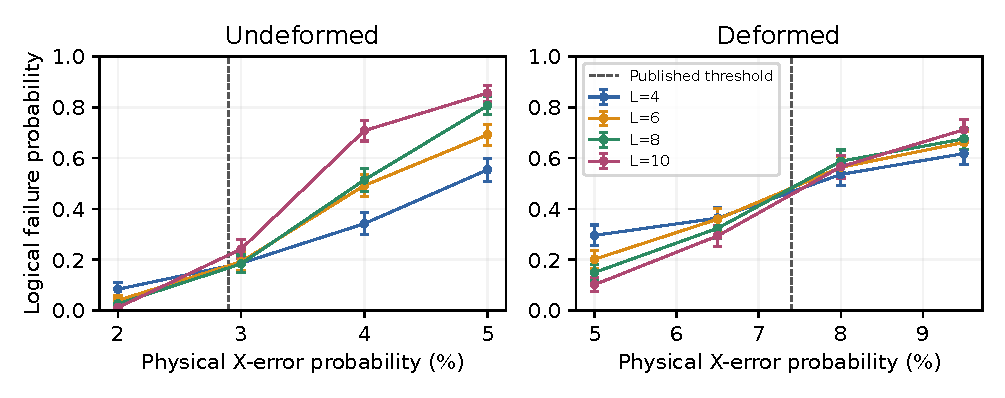
\includegraphics[width=\linewidth]{figures/crossovers.pdf}
\caption{Fresh pure-X logical-failure estimates. Bars are pointwise two-standard-error Monte Carlo bars, not source-comparison or simultaneous intervals. Dashed vertical lines show the printed thresholds; connected points guide the eye. The deformed and undeformed panels use different horizontal ranges to resolve their respective crossovers.}
\end{figure}

\section{Numerical agreement, scope, and uncertainty}
\begin{center}
\begin{tabular}{p{.21\linewidth}rrrrp{.13\linewidth}}
\toprule Quantity & Published & Ours & Deviation & SE & Numerical\\\midrule
Undeformed & 2.9 & 2.388 & -0.512 & 0.104 & mismatch\\
Deformed & 7.4 & 7.570 & +0.170 & 0.274 & mismatch\\
Difference & 4.5 & 5.182 & +0.682 & 0.299 & mismatch\\
\bottomrule\end{tabular}
\end{center}
All entries are percentage points; deviation is ours minus source. Scope is limited for all rows because the production configuration and fit selection are not identified. SE is our conditional bootstrap standard error, not a source SE.
\begin{center}\begin{tabular}{lrrll}
\toprule Quantity & Two-SE band & Adjusted band & Two-SE status & Adjusted status\\\midrule
Undeformed & 0.259 & 0.300 & outside & outside\\
Deformed & 0.597 & 0.705 & inside & inside\\
Difference & 0.698 & 0.816 & inside & inside\\
\bottomrule\end{tabular}\end{center}
Bands are half-widths for the deviation, in pp, conditional on unknown source sampling uncertainty; the rounding bound is included. They are neither numerical-rounding verdicts nor equivalence margins.

Source precision is 0.1 pp for each threshold. A numerical match rounds to the source value; \emph{close} is reserved for one last-place unit after rounding. The difference of two rounded source values has at most 0.1 pp of rounding uncertainty. This is not an estimate of source Monte Carlo uncertainty. Missing original trial counts prevent a two-sample comparison, a statistically established source ranking, or an equivalence conclusion.

We fit the source's equations (3.1)--(3.2),
\[
 y=A+Bx+Cx^2,\qquad x=(p-p_{\rm th})L^{1/\nu},
\]
by unweighted least squares, as described on page 45. The source attributes its finite-size-scaling approach to \citet{tuckett2020}. Our new grid is $p=0.02,0.03,0.04,0.05$ without deformation and $p=0.05,0.065,0.08,0.095$ with deformation. The fit uses three initial values of $\nu$ and selects the smallest residual sum of squares. Parameter bounds and starts are exposed in \repo{simulation/analyze.py\#L16}{analyze.py}.

The 400 binomial bootstrap draws resample each observed cell at its empirical failure rate and refit both arms. \BootstrapStatus\ They measure sampling variation conditional on this graph, decoder, grid and scaling form; they do not include model bias. We report the ordinary two-standard-error comparison first and then a Bonferroni correction for three quantities: both thresholds and their signed difference. The corrected half-width is $z_{1-0.05/6}\,\widehat{\rm SE}$ plus the source rounding bound. Correlation among the three comparisons does not invalidate the Bonferroni bound, although normal bootstrap-SE calibration is approximate. The simultaneous interval for our deformation advantage is \DeltaInterval\ pp, conditional on the chosen fit.

\section{What we did ourselves, and what we took from others}
We independently constructed the periodic vertex/edge and face/edge incidence matrices, sparse min-sum messages, integer-row GF(2) order-zero OSD, Monte Carlo driver, fitting and uncertainty analysis. \repo{simulation/engine.py\#L7}{engine.py} implements the graph and decoder, while \repo{simulation/run.py\#L7}{run.py} records seeds, counts, decoding failures and costs for every condition. The thesis supplies the scientific comparison, noise model, deformation, code family and scaling expression. The BP-OSD method builds on \citet{roffe2020}.

The collaboration's original \texttt{bn3d} is preserved in PanQEC history \citep{bn3d}. We obtained revision \texttt{686560e5d03c2e5d31f6c6260b03756af03a7e93}, the latest pre-submission commit found; it is a historically plausible reference, not a proven production revision. Our validator executes its original dense decoder functions, without redistributing that source. For $L=2,3,4$, both deformation arms, the independent matrices and logical operators match exactly, and all 240 tested syndrome corrections agree. The independent implementation shares the published definitions, test error vectors, NumPy and host with the reference; this is not a second independent end-to-end replication.

NumPy's PCG64 and Python's scalar MT19937 generators independently generate Bernoulli errors, sharing our graph and decoder. \GeneratorStatus\ These 32 comparisons form their own Bonferroni family. Shared decoder bugs would not be detected by this generator check.

Python 3.12.14 provides exact integer bit operations and the standard-library generator \citep{python}. NumPy 2.3.5 provides array arithmetic and PCG64, and SciPy 1.17.0 supplies sparse syndrome multiplication and optimization \citep{numpy,scipy}. Historical qecsim 1.0b9 and NetworkX 2.6.2 are used only to load the reference code's interfaces \citep{qecsim,networkx}. Matplotlib 3.10.8 produces the figures and Pillow 12.3.0 crops source evidence \citep{matplotlib,pillow}. The latter operates on 600-dpi Poppler renders. No SEM estimator is relevant to this binary stabilizer problem.

\section{Assumptions supplied by this replication}
\subsection{Unspecified production settings}
The thesis does not identify production seeds, trial counts, exact package versions, BP iteration count, tie handling, or the fitting window. We use the public reference default of ten BP iterations, its $10^{-8}$ prior regularizer and reliability ordering, and order-zero OSD. NumPy's current quicksort ordering resolves equal reliabilities, with stable sorting examined as a sensitivity; exact historical floating-point and sorting behavior is not established. Python 3.8, requested by the old README, is absent from this environment. We do not label current-runtime reference execution an exact historical-runtime reproduction.

\subsection{Independent trials and perfect measurements}
Each physical qubit receives an independent X error with probability $p$; trials and arm-specific seeds are independent. These are code-capacity experiments with exact syndromes, not circuit-level or repeated noisy-measurement thresholds. Neither the bootstrap nor the code checks extends the finding to correlated noise or hardware.

\subsection{Local scaling and finite resources}
A quadratic scaling form is assumed valid over each selected window. We use bounded numerical optimization to avoid nonphysical exponents, then examine alternative objective functions, removal of extreme lattice sizes and exclusion of probability-grid endpoints. Bootstrap bands exclude finite-size systematic uncertainty. The pilot timed both arms before production; the largest condition took about 0.18 seconds per trial with about 59 MiB resident memory. A 2 GiB address-space limit and 2,400-second CPU limit bound the primary process. Actual production used \RunSeconds\ wall seconds and \RunMemory\ MiB maximum resident memory.

\section{Ambiguities checked and resolved}
\subsection{Printed values versus extracted text}
We rendered source pages 45 and 48 at 600 dpi and visually checked both selected thresholds and every sign/exponent in the fitted equations. The table gives 2.9\% and 7.4\%; the scaling variable contains $p-p_{\rm th}$ and exponent $1/\nu$. \repo{evidence/table3_1.png}{table3_1.png} and \repo{evidence/scaling_equations.png}{scaling_equations.png}, with coordinates and hashes in \repo{evidence/manifest.json}{manifest.json}, preserve those checks. The full source is not redistributed.

\subsection{Channel labels and logical success}
The source uses Z vertex stabilizers and X face stabilizers. We check those operators directly against historical code, rather than relying on prose that sometimes interchanges sector labels. The error/correction pairing is tested through syndrome cancellation and the three logical membranes/strings. \InvalidStatus\ The zero-loop contribution under undeformed pure-X noise is a structural consequence of the selected channel, not discarded failed trials.

\subsection{Iteration and fitting choices}
\begin{center}\begin{tabular}{lrrr}
\toprule Fit choice & Undeformed (\%) & Deformed (\%) & Difference (pp)\\\midrule
Primary least squares & 2.388 & 7.570 & +5.182\\
Binomial likelihood & 2.487 & 7.608 & +5.121\\
Exclude highest p & 2.805 & 7.614 & +4.809\\
Exclude lowest p & 2.850 & 7.215 & +4.365\\
Exclude L=4 & 2.134 & 7.859 & +5.724\\
Exclude L=10 & 2.763 & 7.331 & +4.567\\
numpy generator only & 2.239 & 7.444 & +5.205\\
stdlib generator only & 2.534 & 7.704 & +5.171\\
\bottomrule\end{tabular}\end{center}
\begin{center}\begin{tabular}{llrrr}
\toprule L & Arm / p & 10 iterations & 100 iterations & Stable ties\\\midrule
4 & Undeformed / 0.03 & 0.220 & 0.230 & 0.216\\
4 & Deformed / 0.08 & 0.526 & 0.536 & 0.526\\
6 & Undeformed / 0.03 & 0.204 & 0.188 & 0.202\\
6 & Deformed / 0.08 & 0.508 & 0.544 & 0.512\\
\bottomrule\end{tabular}\end{center}
Iteration entries are logical-failure probabilities, with 500 trials per entry. The three diagnostic columns share error seeds, but differ from main-grid seeds. Stable ties uses ten iterations with stable reliability sorting. These are exploratory finite-point checks, not threshold estimates or significance claims.

We rerun 100 BP iterations at $L=4,6$, $p=0.03$ undeformed and $p=0.08$ deformed, retaining the original primary run. Those diagnostic runs share error seeds with separate ten-iteration and stable-sorting baselines; they are not a full threshold re-estimation. We also fit binomial likelihood with a separate optimizer, drop $L=4$, drop $L=10$, exclude each probability-grid endpoint, and fit each generator independently. Removing a probability endpoint moves the undeformed estimate from 2.388\% to 2.805--2.850\%, explaining much of the primary numerical gap without changing the decoder. Stable reliability ordering is also checked at the same finite points. These alternatives probe remaining causes of numerical differences and are exploratory; none silently replaces the primary estimator. A repeated implementation check cannot resolve an unspecified production configuration.

\section{What remains unresolved}
The principal remaining gap is whether this historically plausible decoder configuration is the one used for the printed numbers. Candidates, in descending practical priority, are (1) original fitting window and finite-size effects, examined by changing objective and size range; (2) decoder production settings and historical tie behavior, partly examined by the 100-iteration and stable-sorting reruns and dense-reference validation; and (3) Monte Carlo variation, examined by two generators and 400 bootstrap draws. The sensitivity table records how much the first candidate moves each threshold; the iteration table records the second candidate's finite-point effect. These checks do not prove a cause or establish author error.

Our side was checked for source transcription, channel identification, metric, uncorrected syndromes, original algorithm, independent implementation, generator effects and optimizer dependence. The source's actual trial-level production archive---including job inputs, software environment and the fit selection---is the single artifact that would settle the largest remaining uncertainty. Until that is available, the comparison is a limited reconstruction, with conditional uncertainty and no claim that the source values are wrong. The source itself describes the numerical study as preliminary and calls for refined scaling and error bars on pages 57--58.

\section{Code and source availability}
The dated rows below are copied from \repo{availability.md}{availability.md}; they distinguish obtained material from searches that did not identify a relevant record. No author contact was made.
\begin{longtable}{p{.21\linewidth}p{.12\linewidth}p{.59\linewidth}}
\toprule
Place checked & UTC date & Result\\
\midrule\endhead
Dissertation and author-hosted manuscript & 2026-10-30 & Obtained complete 66-page PDF from artix41/artix41.github.io at \nolinkurl{b4f401e0c12b44be4c69318e0015f70d8a3d3f98}; hash in evidence/manifest.json. Thesis names bn3d but gives no pinned production revision or trial counts.\\
Author GitHub account artix41 & 2026-10-30 & All 47 returned public repositories shallow-cloned; individual revisions and outcomes in results/author-clones.json. Filename and targeted source search did not identify a thesis production-results bundle. This is a snapshot search, not a claim about private or deleted material.\\
PanQEC collaboration repository & 2026-10-30 & Full history obtained. Historical bn3d at \nolinkurl{686560e5d03c2e5d31f6c6260b03756af03a7e93} is the last pre-submission commit found. Arthur Pesah authored decoder commits. Code executed as an independent reference; exact production identity remains unverified.\\
OSF & 2026-10-30 & Web-index query for Arthur Pesah plus OSF did not locate a project for this dissertation. No project identifier given in thesis; no claim of exhaustive absence.\\
GitLab & 2026-10-30 & Web-index query returned an unrelated ENSTA scheduling project/login page, not a quantum-decoding supplement. No relevant project identified.\\
Zenodo & 2026-10-30 & Web-index query for Arthur Pesah, 2021 and Zenodo did not identify a dissertation result archive. No relevant record identified.\\
Historical package/runtime check & 2026-10-30 & qecsim 1.0b9 and networkx 2.6.2 obtained and used for reference validation. Python 3.8 is not installed; historical NumPy/SciPy versions and seeds are not pinned by source. Executed under Python 3.12.14, NumPy 2.3.5, SciPy 1.17.0; exact historical runtime not established.\\
\bottomrule
\end{longtable}


\section{Compliance record}
These rows are copied from \repo{compliance.md}{compliance.md}. The approved layout is preserved without subject-specific style changes; quantum methods replace the inapplicable SEM engine, with preflight justification and separate validation.
\begin{longtable}{p{.23\linewidth}p{.70\linewidth}}
\toprule
Requirement & Execution and limit\\
\midrule\endhead
New scheduled quantum dissertation & Slot 2; prior studies/register/all-state PRs checked against current master. Pesah 2021 MRes is distinct from excluded Higgott, Denys, and the inaccessible Pesah 2026 PhD.\\
Full source and bounded headline & Complete 66-page text read, selected methods/results visually checked. Selected substantive pure-X cubic threshold comparison in Table 3.1/Figure 3.5. Pure-Z, rhombic, circuit noise, and SweepMatch claims remain outside this study.\\
Engine preflight & Preflight accepted justified quantum departure: binary stabilizer/BP-OSD decoding is not an SEM estimand. R/lavaan/OpenMx unavailable and scientifically inapplicable.\\
Independent checks & Independent incidence construction and sparse/integer decoder compared with historical dense source: 240 identical syndromes, sizes 2/3/4, both deformation arms. Shared source definitions, error inputs, NumPy, and machine; partial implementation independence only. PCG64 and standard-library MT19937 provide separate Monte Carlo generators, sharing decoder and graph.\\
Resource pilot & 20 shots per arm at L=4/6/8 and 10 per arm at L=10. Largest pilot about 0.18 seconds/shot and 59 MiB resident memory. Production bound: one process, 2400 CPU seconds, 2 GiB address space; checkpoints per condition.\\
Comparable estimand & Perfect-syndrome independent pure-X Pauli channel, periodic cubic sizes 4/6/8/10, Hadamard on x edges, full logical failure, order-zero OSD. Both source arms are run. Comparison is limited by missing production configuration, counts, seeds, runtime pins and fitting window.\\
Supplied defaults & Historical public default 10 BP iterations; 100-iteration sensitivity at L=4/6. Source epsilon 1e-8 retained. Selection moved from initially screened doctoral works to an accessible MRes dissertation that bears the requested dissertation designation; no PhD status or user-specific Pesah selection is implied. New probability grid brackets each crossover; 250 shots per generator per condition.\\
Agreement and uncertainty & Source thresholds printed to 0.1 percentage point; half-up rounding evaluated independently of scope and uncertainty. Three threshold comparisons form a Bonferroni family. Unknown source uncertainty makes source bands conditional. A separate 32-cell family tests generator differences.\\
Signed effects & Primary contrast is deformed minus undeformed threshold in percentage points; positive favors deformation. Ours-minus-source deviations use a separate field. Inventory and coverage helper checks required.\\
Source evidence and rights & 600-dpi table and equation crops, hash/coordinate manifest, no complete dissertation or third-party source in git. New original Python code follows repository scope; imported research evidence is excluded.\\
Manuscript and delivery & Approved preamble retained, main manuscript leads with selected headline and limits. Final artifact/reproduction revisions, rendered-PDF review and remote byte hashes recorded separately after build. Master navigation is prospective until merge.\\
\bottomrule
\end{longtable}


\section{Next steps}
Obtain the production archive just named, then rerun the selected grid with its exact settings and reapply both the source estimator and the independent fitting diagnostics. Larger sizes and a preregistered, narrower crossover window could test finite-size bias, but would be a new computational study. The current source uncertainty cannot be filled in by assuming the original run was effectively noiseless.

\bibliographystyle{plainnat}
\bibliography{references}

\appendix
\section{Artifacts and execution}
The historical repository baseline is \texttt{e2b553c06c872d8008061a26d05831e572e54789}. The runnable reproduction revision is \ReproductionRevision. The immutable reproduction revision is available on GitHub for review. New \texttt{master} navigation links in this manuscript await merge. The complete commands, prerequisites, output paths and seeds are in \repo{README.md}{README.md}. Main manuscript source is \repo{paper/manuscript.tex}{manuscript.tex}, with \repo{paper/references.bib}{references.bib} and \repo{paper/approved-preamble.tex}{approved-preamble.tex}.

\begin{longtable}{p{.24\linewidth}p{.30\linewidth}p{.38\linewidth}}
\toprule Claim/artifact & File & Regeneration from study root\\\midrule\endhead
Primary 16,000 trials & \repo{results/primary.json}{primary.json} & \texttt{python simulation/run.py --output results/primary.json}\\
Original-source agreement & \repo{results/validation.json}{validation.json} & \repo{simulation/validate.py}{validate.py}; source checkout and historical dependencies required\\
Thresholds, uncertainty, coverage & \repo{results/analysis.json}{analysis.json} & \texttt{python simulation/analyze.py}\\
Iteration sensitivity & \repo{results/iterations100.json}{iterations100.json} & \repo{simulation/run.py}{run.py} with \texttt{--iterations 100 --sizes 4 6 --sensitivity}\\
Source evidence & \repo{evidence/manifest.json}{manifest.json} & \repo{simulation/crops.py}{crops.py} with external full PDF path\\
Figures and manuscript tables & \repo{simulation/paper_assets.py}{paper_assets.py} & \texttt{python simulation/paper\_assets.py}\\
Engine departure & \repo{results/preflight.json}{preflight.json} & Skill \href{https://github.com/alectionary/vibe-math/blob/master/.agents/skills/replication-paper/scripts/preflight.py}{\nolinkurl{preflight.py}} with \repo{preflight-departure.json}{preflight-departure.json}\\
Main PDF & \repo{paper/pure_x_thresholds_of_deformed_cubic_codes__replication_of_pesah_2021.pdf}{pure_x_thresholds_of_deformed_cubic_codes__replication_of_pesah_2021.pdf} & \repo{paper/build.sh}{build.sh}; requires pdfLaTeX and BibTeX\\\bottomrule
\end{longtable}
\end{document}
